\documentclass[12pt]{article}
\usepackage{amsmath}
\usepackage[utf8]{inputenc}
\usepackage[T1]{fontenc}
\usepackage[danish]{babel}
\renewcommand{\rmdefault}{ptm}
\usepackage[pdftex]{graphicx}

\title{IT-løsning til Tolkeservice}
\author{Omar Khalidan - [xx-xx-xx]\\
     Morten Trolle Nielsen - [14-06-79]\\ \\
    Instruktor: Andreas Frisch\\ \\
Projekt i systemudvikling 2014 (ProjDat2014)}

\begin{document}
\maketitle
\thispagestyle{empty}
\newpage
\tableofcontents
\newpage

\section{Abstract}
Dette er anden delrapport i faget Systemudviking. Vores udgangspunkt er første
delrapport, som vi her udvikler og udbygger. Vi vil foresætte arbejdet med og
præsentationen af den IT-løsning, som vi har udviklet til kunden; tolkeservicen
K. Translation. Specielt vil vi fokusere på modelleringen af systemet. Vi vil 
præsentere anvendelsesområdet og problemområdet; både med tekst og UML-diagrammer.
Det skal resultere i en bedre og umiddelbar forståelse af vores påtænkte it-løsning.
Derefter vil vi også med afsæt i første delrapports kravspecificering videreudvikle
denne og se på de funktionelle og nonfunktionelle krav. Vi vil tage modelleringen
et skridt videre ved hjælp af use-cases, så vi kan understøtte vores modellering med
konkrete eksempler på brug af systemet. \\
Vi vil afslutte denne anden delrapport med to korte referater og efterfølgende
analyse og perspektivering af de to artikeler, der er et krav til rapporten.\\
Vi er selv førsteårs datalogistuderende ved Københavns Universitet, og det
forudsættes, at læseren befinder sig på samme læringsniveau eller højere, idet
der undervejs vil forekomme adskillige fagspecifikke termer. 

\newpage

\section{Problemformulering}

\emph{”Hvordan konstruerer man et bookingsystem til en tolkevirksomhed, som
formindsker tidsspilde og fejl ? Og hvordan kan dette gøres på en brugervenlig
måde, så virksomhedens samarbejdspartnere enkelt og simplet kan tilgå systemet 
uden for meget tidsspilde ?”}\\

Tolkeservicen K. Translation er et lille, enmands tolkebureau med speciale i arabiske 
sprog. Indehaveren af bureauet er , og hun er som sagt både leder og eneste
medarbejder i foretagendet. Hendes kunder er offentlige myndigheder som
politiet og anklagemyndigheden og private aktører som advokatbureauer og
forskellige virksomheder. Disse instanser kontakter K. Translation, når de har
behov for en tolk til konkrete sager eller ved andet forefaldende
tolkearbejde, og der laves en aftale. Det kan både være aftaler to eller tre uger 
ude i fremtiden, eller det kan være aftaler med kortere frist ved mere presserende 
sager.\\
K. Translation (KT) har i længere tid ønsket et it-system, som kan
afhjælpe lidt af den daglige travle arbejdsbyrde. Derfor tog ejeren af KT
kontakt til os, og anmodede om et møde omkring dette problem. Det første møde fandt 
sted fredag den 21. marts, og vi blev enige om at begynde et samarbejde, der
skal resultere i et færdigt kalender- og bookingssytem til KT og KT's kunder.
Kunden præsenterede os for en liste af de funktioner, som hun ønsker, at det nye system
skal kunne levere. For det første ønskes der en hjemmeside, hvor KT's kunder
kan logge på systemet med deres EAN-nummer. Da vi bl.a. snakker om offentlige
myndigheder som politi og anklagemyndighed, skal login systemet fremstå
professionelt og sikkert. Der skal være en tilhørende database indeholdende
alle KT's kunder, og det skal være muligt løbende at tilføje kunder til
databasen. \\
Når KT's kunde har logget på systemet, skal vedkommende præsenteres for en
kalender opslået på dags dato med mulighed for visning af de næste to til tre
uger. Det er KT's holdning og erfaring, at der ikke forekommer aftaler længere
end tre uger ude i fremtiden; derfor denne begrænsning. KT's kunde skal i
kalenderen kunne se alle de tidspunkter, hvorpå det er muligt at booke en
aftale med K. Translation. Disse ledige tidspunkter kan evt. markeres med
grønt. Allerede indgåede aftaler markeres med rødt for at tydeliggøre
denne forskel. Når KT's kunde har besluttet sig for en dato og et tidspunkt,
taster vedkommende dette ind i systemet, og aftalen gemmes i databasen og
vises herefter i kalenderen. Det er vigtig for KT's ejer, at hendes
samarbejdspartnere ikke skal bruge alt for lang tid på at booke en aftale, så
enkelhed og intuitivitet skal prioriteres højt.\\



\section{Anvendelsesområde}
Vi vil i de næste afsnit kigge på to centrale dele af enhver modellering;
nemlig anvendelses- og problemområdet. Vi begynder her med en analyse af
anvendelsesområdet, og for overskuelighedens skyld præsenterer vi det først
ved hjælp af et UML-diagram. Se figur \ref{fig:anvend}.\\

\begin{figure}[!ht]
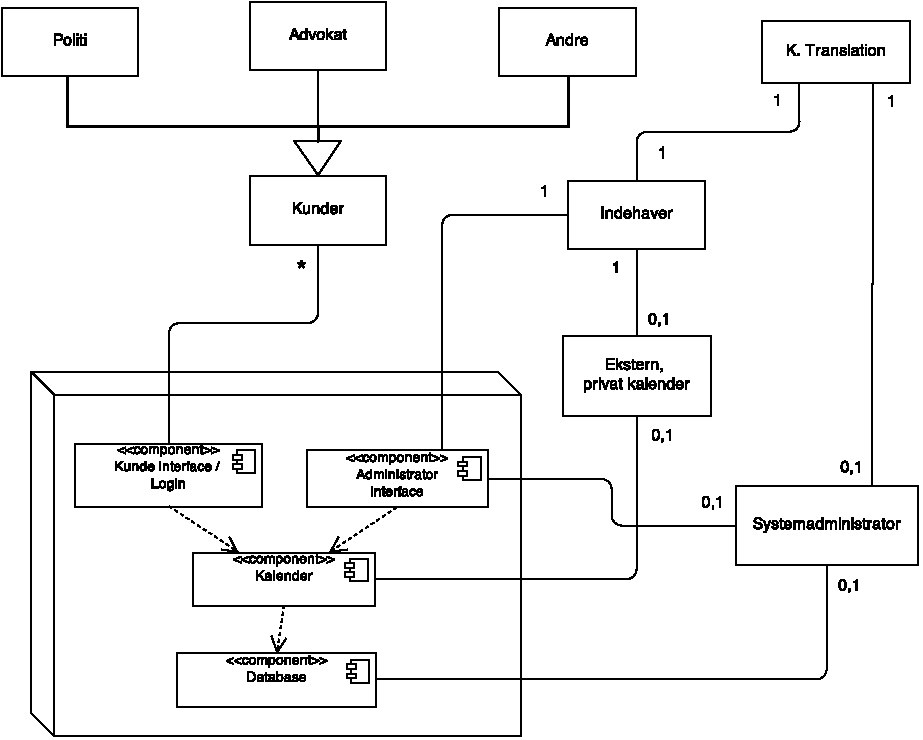
\includegraphics[width=12cm, height=11cm]{anvendelsesomr.pdf}
\caption{UML-diagram over anvendelsesområdet}
\label{fig:anvend}
\end{figure}

Det skal dog præciseres, at det store kvadrat i nederste venstre hjørne i figur
\ref{fig:anvend} ikke hører til anvendelsesområdet. Det er et high-level
billede af problemområdet, som her er medtaget for at binde de to områder sammen,
og som behandles indgående i næste afsnit.\\ 
Umiddelbart er anvendelsesområdet meget begrænset. Vi har fundet følgende
klasser, der skal modelleres i anvendelsesområdet:

\begin{itemize}
\item K. Translation med indehaver (som samtidig er eneste medarbejder)
\item Systemadministrator kos K. Translation
\item K. Translations kunder som politi, advokater, etc.
\item Eksternt, privat kalendersystem 
\end{itemize}

K. Translations indehaver, som samtidig er den eneste medarbejder, skal som
den første modelleres i systemet. Hun skal bruge kalenderen og
bookingssystemet i sit daglige arbejde, og hendes ønske er, at kunne kombinere
hendes private kalender med vores it-løsning, så hun har alle sine aftaler
samlet et sted. Derfor har vi modelleret hende som indehaver af K.
Translation og bruger af kalenderen, men vi har samtidig udvidet modellen med
en ekstern kalenderklasse mellem indehaveren og systemet, hvor hendes private
aftaler ligger, og hvor den eksterne kalender kan synkronisere med vores
bookings- samt kalendersystem og overføre de private aftaler. Det skal dog
siges, at vi på nuværende tidspunkt er meget usikre på denne funktion, og at
vi potentielt må fortælle K. Translation, at dette ligger uden for vores
formåen, så vi er påpasselige med at stille hende for meget i udsigt. Derfor
har den også i UML-diagrammet fået multiplicitet 0, 1, da vi højest regner med
1 ekstern kalender, der skal integreres. Det kunne godt gå hen og blive en stor
og kompliceret opgave, så derfor får den også i første omgang en lavere prioritet 
end andre mere tilgængelige ønsker. Se evt. afsnittet om projektplan.\\
Vi har i UML diagrammet givet indehaveren af KT multiplicitet 1.
Man kunne sagtens forestille sig flere ejere af bureauet, men vi har taget
udgangspunkt i den nuværende situation, og der er ikke umiddelbart udsigt til 
nogen ændringer. Selvom indehaveren ikke besidder it-kundsskaber ud over det
almindelige, har vi i erkendelse af, at hun også er eneste medarbejder, i
UML-diagrammet givet hende adgang til administrationsinterfacet, da hun sikkert
vil komme i en situation, hvor hun selv er nødt til at tilgå systemet med alle
rettigheder for at ændre eller oprette nye kunder. \\
Hvis vi skal foresætte modelleringen af anvendelsesområdet, så er der en
Systemadministratorklasse associeret til K. Translation. Indehaveren af KT
er ganske almindelig it-bruger, og her snakker vi om mail, netbank, facebook,
etc, men er ikke it-kyndig udover dette. Derfor er vi nødt til at modellere en
systemadministrator, der har overblik over systemet, og som kan yde support,
hvis der opstår problemer. Hvis det færdige system ikke kommer til at ligge på
en intern server hos KT, men ender med at blive hosted af en ekstern udbyder 
af serverplads, så vil nødvendigheden af denne klasse mindskes betragteligt,
men der vil altid være et vist behov for central systemadministration hos KT i
tilfælde af ændringer i kontaktinformation eller kalenderbrug med dertil
hørende ændringer i kodebasen og efterfølgende nye upload til serveren. K.
Translation må selv tage stillig til, hvor meget systemadministration der er
nødvendig efter afleveringen og implementeringen af systememet, men vi vil
naturligvis indgå i en dialog med hende omkring dette emne, når det bliver
aktuelt. \\
Den sidste klasse, der skal modelleres i anvendelsesområdet, er KT's kunder og
samarbejdspartnere. Denne klasse er omdrejningspunktet for hele systemet, da
en af hovedpræmisserne for vores it-løsning er, at KT's kunder på en hurtig og
overskuelig måde kan booke en aftale med tolkeservicen. Kundegrundlaget er  
offentlige myndigheder som politi, ministerier og hospitaler samt private
aktører som advokater og andre samarbejdspartnere. Når de møder hjemmesiden, skal
de kunne tilgå kalenderen via et loginsystem med deres EAN-nummer og derfra
føres videre til selve kalenderen, hvor der kan bookes en aftale. Vi må
forvente, at kundesegmentet har meget svingende it-kundsskaber, men at de i
kraft af deres daglige arbejde er vant til at arbejde med diverse login- og 
kalendersystemer, der findes overalt i f.eks. den offentlige sektor. \\

\section{Problemområde}
Efter at vi har modelleret tilgangen til it-systemet gennem
anvendelsesområdet, er turen nu kommet til systemets hjerte: problemområdet. 
Det er her, vi efter modelleringen skal implementere de løsninger, vi finder
på KT's ønsker. For at binde modelleringen sammen går alle klasserne fra 
anvendelsesområdet igen i problemområdet. Vi præsenterer igen for
overskuelighedens skyld først et UML-diagram over området. Se figur 
\ref{fig:problem}. Dernæst kommer der en kort opsummerende liste med klasserne 
efterfulgt af et længere forklarende afsnit.  

\begin{figure}[!ht]
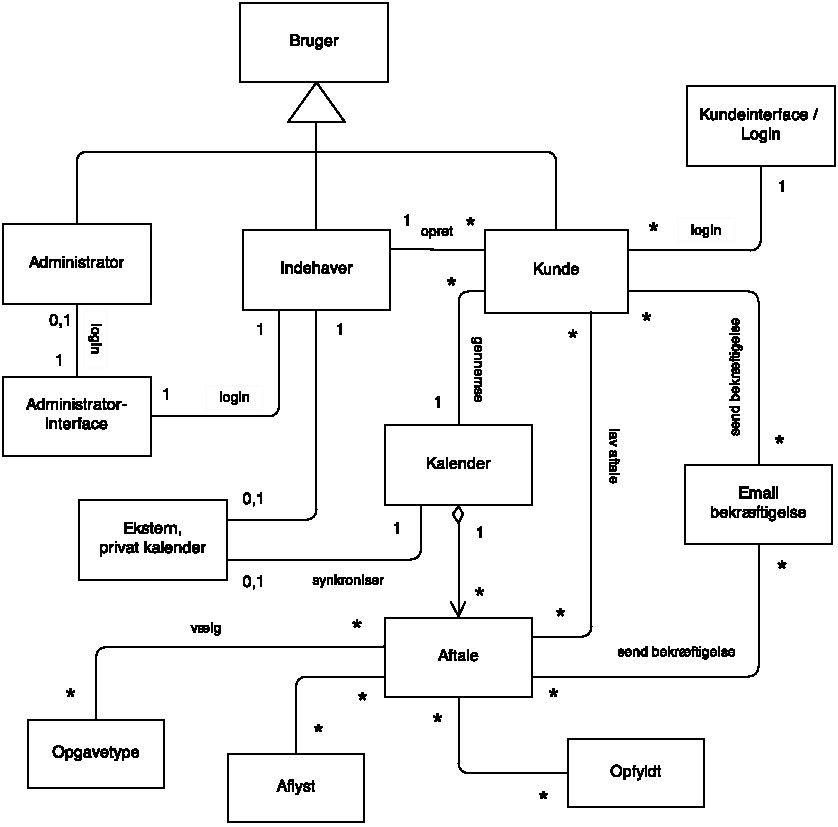
\includegraphics[width=12cm, height=12cm]{problemomr.pdf}
\caption{UML-diagram over problemområdet}
\label{fig:problem}
\end{figure}

Her følger en liste af de klasser vi har identificeret i problemområdet:

\begin{itemize}
\item Bruger: Kunde, administrator, indehaver. Går igen fra
	anvendelsesområdet
\item To interfaces. Et til kunderne og et til administratoren
\item Kalenderen, som kunderne kan bruge, når de skal finde en ledig tid, og
	som KT's indehaver kan bruge i sit daglige, travle arbejde
\item Aftale. Kunderne booker en aftale i kalenderen.
\item En aftale kan både være aflyst og opfyldt, hvis den ikke længere er
	aktuel
\item Når kunden har booket en aftale, sendes der en bekræftende email tilbage
	til kunden med det aftalte tidpunkt
\item KT's indehaver har et ønske om at kunne synkronisere hendes eksterne,
	private kalender med vores it-løsning
\end{itemize}

Vi begynder denne gennemgang af problemområdet med de to interfaces, hvor
brugerne først møder systemet. Systemadministratoren får sit eget selvstændige
interface, idet vedkommende skal kunne tilgå systemet med samtlige
rettigheder. Som vi også nævnte under gennemgangen af anvendelsesområdet, så
skal KT's indehaver alene i kraft af, at hun er eneste medarbejder, også have
adgang til systemet gennem administratorinterfacet. Det betyder også, at vi efter
implementeringen er nødt til at undervise hende grundigt i brugen, og at vi
fabrikerer nogle enkle og præcise manualer, hun efterfølgende kan slå op i.
KT's kunder vil også blive præsenteret for et login interface, når de
navigerer til hjemmesiden. Efter login vil der være adgang til kalender og
bookingsystemet. \\
Omdrejningspunktet i problemområdet må siges at være kalenderen, da hele
systemets berettigelse hviler på denne. Vi skal have fundet en eller anden
kalenderform, der passer til opgaven og KT's arbejdsgange. Indehaveren af K.
Translation har som udgangspunkt fortalt, at der ikke forekommer aftaler længere
end 2-3 uger ude i fremtiden, men det vil også være for meget for en
almindelig computerskærm at skulle vise to eller tre hele kalenderuger med
aftaler, så derfor er vi nødt til at finde et acceptabelt kompromis på,
hvordan kalenderen skal præsenteres. Vi kunne begynde med at vise kunden dags 
dato og inkorporere søgefunktioner på dag, uge og klokkeslet, men det endelige
design er på nuværende tidspunkt ikke fastlagt.\\
Det er også et krav til kalenderen, at kunden let kan skelne mellem ledige
tidspunkter og allerede bookede aftaler ved hjælp af et farvesystem. Her vil
ledige tidspunkter være markeret med grøn skrift og aftaler med rød skrift. \\
Dette fører modelleringen af problemområdet videre til aftale klassen. Der vil 
være en naturlig sammenhæng mellem kalender og aftale, og derfor er de
sammenkoblet ved aggregering. En kunde kan lave en eller flere aftaler på
samme tid, og vedkommende vil efter hver indgået aftale automatisk modtage en 
bekræftende email med dato og tidspunkt. Dette ses til højre i UML-diagrammet,
hvor emailen autogeneres og sendes tilbage til kunden. 

\section{Kravspecifikation}
\subsection{Funktionelle krav}
\subsection{Non-funktionelle krav}
\section{Softwarearkitektur}

\section{Use-cases}
\section{Projektplan}

\section{No silver bullit}
\section{ den anden artikel}

\end{document}

